
La detección de muones en este proyecto es realizada mediante un detector de partículas inspirado en los detectores sTGC del experimento ATLAS, en CERN. La sigla significa ''small Thin Gap Chamber", y forman parte de un espectrómetro de muones para conocer momento y trayectoria de estas partículas. Esta información permite la reconstrucción de eventos asociados a colisiones de partículas. La figura \ref{img:atlas-layout} ilustra la ubicación de los detecotres de muones dentro del espectrómetro de ATLAS, en el costado superior derecho. La figura \ref{img:atlas-tgc} corresponde a una fotografía de los detectores TGC involucrados en este espectrómetro.

\begin{figure}[h]
	\centering
	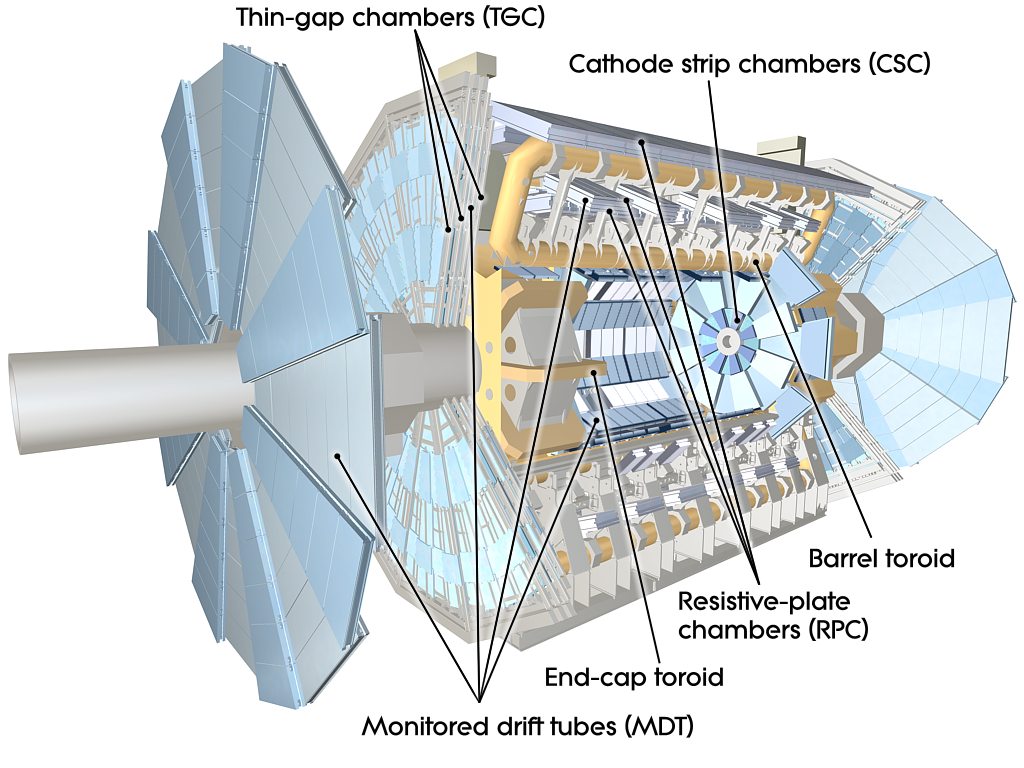
\includegraphics[scale=0.3]{atlas-muon-spectrometer-layout.png}
	\caption{Diagrama del espectrómetro de muones en el experimento ATLAS\cite{AtlasMuonDiagram}.}
	\label{img:atlas-layout}
\end{figure}

\newpage
\begin{figure}[h]
	\centering
	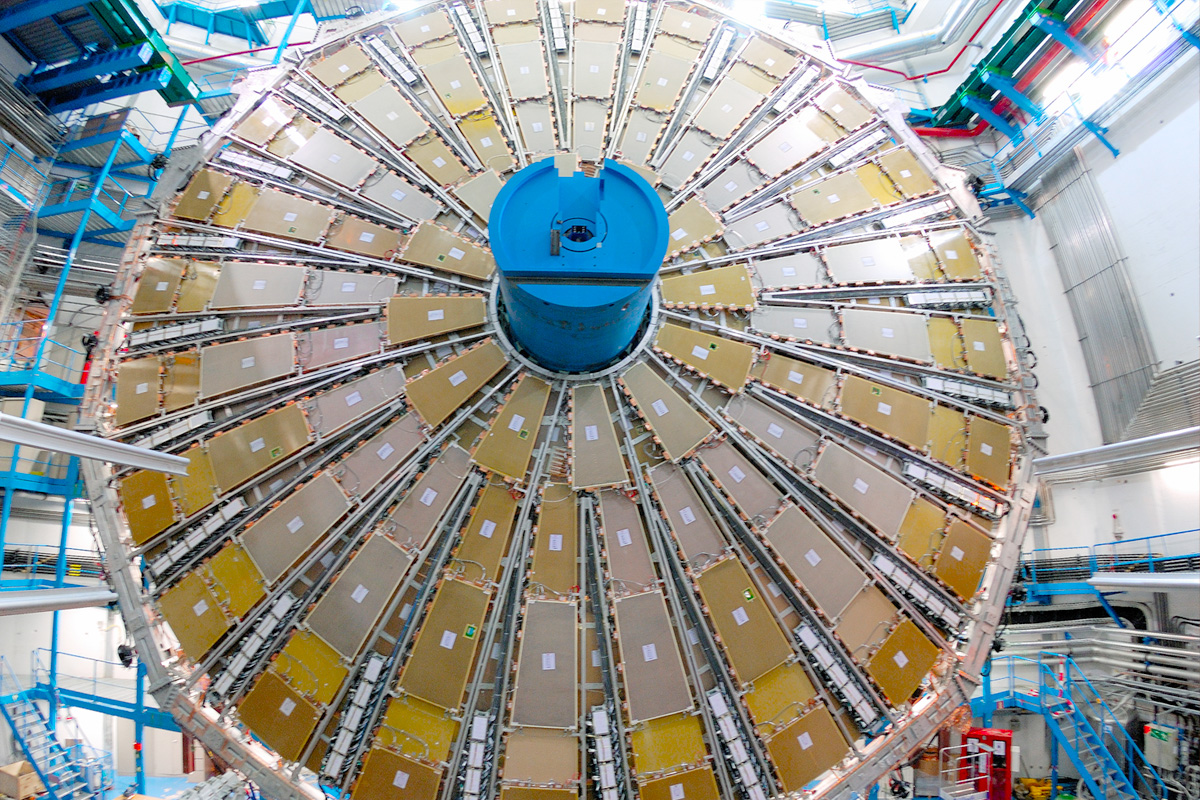
\includegraphics[scale=0.3]{atlas-muon-tgc.jpg}
	\caption{Fotografía del los detectores sTGC en el espectrómetro de muones del experimento ATLAS\cite{AtlasMuonSpect}. El diámetro de este dispositivo es de aproximadamente 24 metros.}
	\label{img:atlas-tgc}
\end{figure}

\begin{figure}[h]
	\centering
	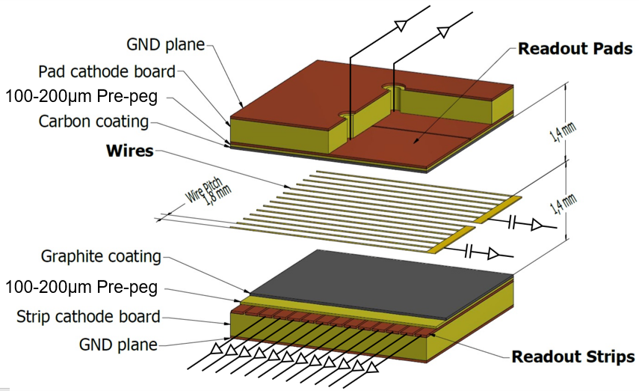
\includegraphics[scale=0.7]{tgc-structure.png}
	\caption{Estructura interna de un detector TGC\cite{Chapman2014}.}
	\label{img:stgc-structure}
\end{figure}

\newpage
\section{Estructura}

	Un TGC está compuesto por dos planos de grafito (cátodos), con múltiples cables en medio (ánodos), como se observa en la figura \ref{img:stgc-structure}. Recubriendo el exterior de ambos cátodos se ubican capas aislantes que los separan de zonas conductoras. Estas son llamadas ``\textit{pads}'' en la cara superior y ``\textit{strips}'' en la cara inferior del detector. Los cables se encuentran orientados perpendicularmente respecto a los \textit{strips}.
	
	Al interior del detector, entre los planos de grafito, se infiltra un gas compuesto por dióxido de carbono y n-pentano. Mediante la aplicación de alto voltaje, se genera un campo eléctrico entre ánodos y cátodos. La figura \ref{img:stgc-field} representa un corte transversal de un detector y sus lineas de cambo eléctrico desde ánodo (cables) hasta cátodos (lámina de grafito superior e inferior).
	
	El paso de muones a través del detector genera la ionización del gas y la liberación de electrones, los cuales son captados por los cables del detector gracias al campo eléctrico.
	
	El flujo de electrones en el gas ionizado genera pulsos de corriente en los cables, produciendo a la vez diferencias de potencial en los cátodos. Estos últimos interactúan con los \textit{pads} y \textit{strips} en el exterior del detector, en los cuales aparecen pulsos de corriente con polarizad inversa respecto a los cables.
	
	La amplitud de los pulsos generados en el detector será mayor en torno a la zona del evento ionizante y menor en zonas lejos de ella. Esto permite relacionar la posición y energía de la partícula con las amplitudes de los pulsos en cada \textit{strip} o cable.
	
	\begin{figure}[h]
		\centering
		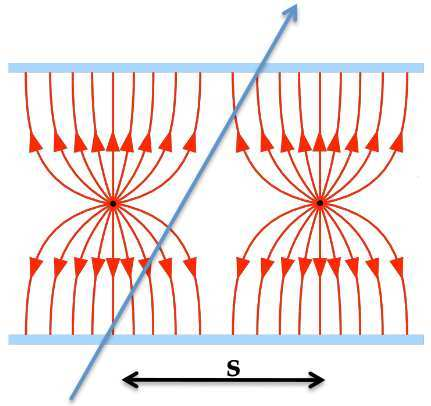
\includegraphics[scale=0.3]{stgc-transversal.png}
		\caption{Lineas de campo eléctrico observadas en un corte transversal de los cables y cátodos del detector. Los cátodos se ilustran en celeste, los cables se representan en negro, y las lineas de campo corresponden a las flechas de color rojo\cite{GEMTracker}.}
		\label{img:stgc-field}
	\end{figure}

\newpage
\section{Detector sTGC utilizado}
	En ATLAS se leen señales provenientes de cátodos y ánodos a la vez. Esto permite trazar coordenadas de posición para cada evento, ya que los \textit{strips} son perpendiculares a los cables. En este proyecto de titulación se leerán solo las señales provenientes de los \textit{strips}, por los que solo se estaría midiendo un eje de posición. 
	
	Para agregar un eje adicional, se reemplazan los \textit{pads} de la cara superior por \textit{strips} perpendiculares a los del plano contrario. Así se logra tener información bidimensional del paso de una partícula leyendo solo las señales provenientes de \textit{strips}. La figura \ref{img:stgc-mini-estructura} ilustra la composición del detector capa por capa y detalla la orientación de cables y \textit{strips}.
	
	En particular, el detector utilizado cuenta con 8 \textit{strips} útiles por lado, de 10 centímetros largo y 1 centímetro de ancho cada uno. Una fotografía de este detector se incluye en la figura \ref{img:foto-mini-stgc}. Se utilizan 3000 $V_{DC}$ entre cátodos y ánodos para generar el campo eléctrico, limitando la corriente a 50uA. El gas en su interior puede ser dióxido de carbono puro, con el compromiso de generar mayor cantidad de descargas no asociadas a muones.
	
	\begin{figure}[h]
		\centering
		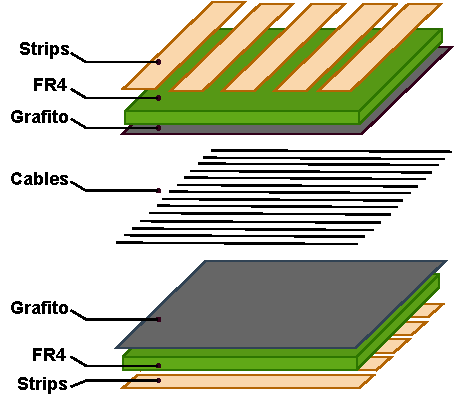
\includegraphics[scale=1]{stgc-mini-estructura}
		\caption{Estructura interna de un detector sTGC adaptado para este proyecto de titulación. El gas es contenido entre ambas capas de grafito (cátodos). Los cables internos corresponden a los ánodos.}
		\label{img:stgc-mini-estructura}
	\end{figure}
	
\newpage
	\begin{figure}[h]
		\centering
		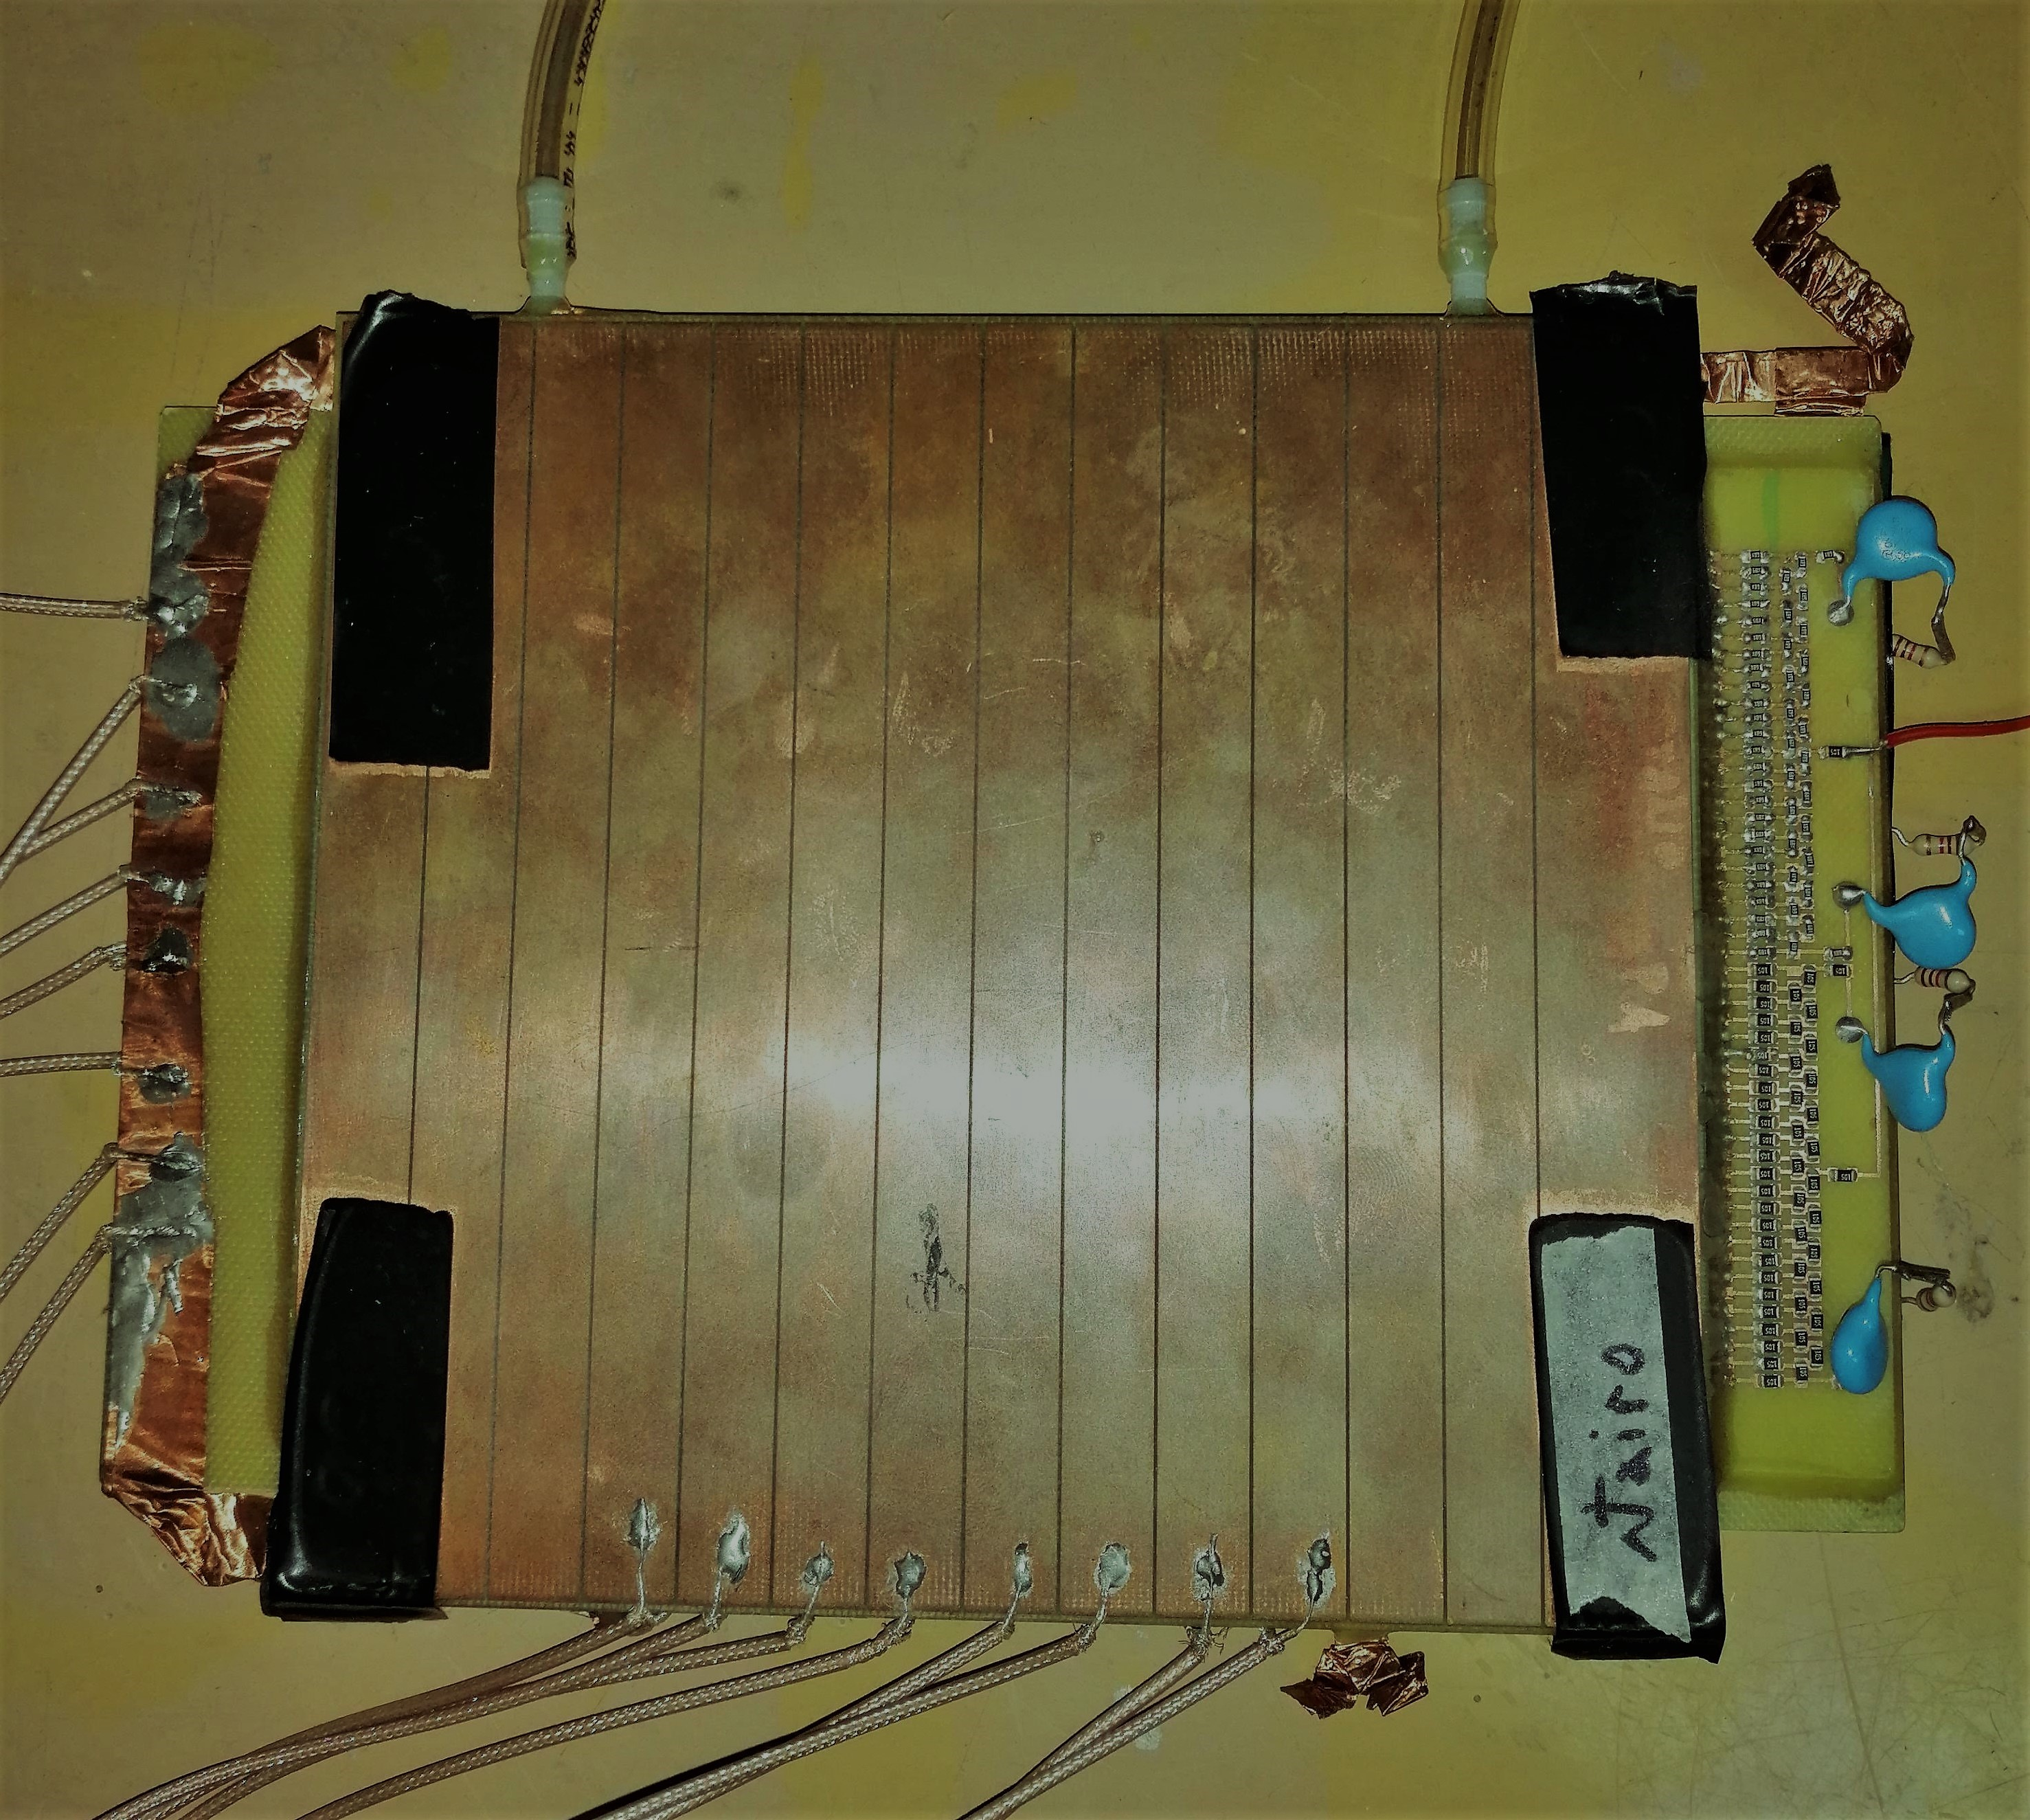
\includegraphics[scale=0.09]{mini-stgc.jpg}
		\caption{Vista superior del detector utilizado. Arriba se observan tubos para el flujo de gas. Abajo se ubican 8 cables coaxiales conectados a los \textit{strips} centrales de una cara del detector. A la izquierda están situados los otros 8 cables correspondientes a los \textit{strips} de la cara inferior. En el costado derecho se observa una red resistiva ponderadora para la lectura de los cables internos del detector, los cuales no serán utilizados en este proyecto.}
		\label{img:foto-mini-stgc}
	\end{figure}

\section{Procedimiento de Operación y Pruebas}
	Antes de poner en marcha mediciones o experimentos con un nuevo detector, se deben realizar ajustes, caracterizaciones y pruebas que permitan corroborar el correcto funcionamiento del dispositivo. Para esto, se recomienda llevar a cabo una secuencia de experimentos con el fin de comprobar el funcionamiento de cada canal y medir el ruido base, la frecuencia de detección y las amplitudes medias esperadas.

	\subsection{Dispositivos para lectura de señales}
		Para observar los pulsos captados por el detector, es necesario contar con un sistema de lectura adecuado. Este dispositivo deberá poseer una impedancia de entrada adecuada para evitar reflexiones, así como también deberá contar con una ganancia tal que permita medir sin problemas las señales captadas con un osciloscopio, digitalizador o un sistema para adquisición de datos.
		
		Un ejemplo es la tarjeta ASD, que será utilizada en este proyecto de titulación. Está diseñada para la correcta lectura de \textit{strips} y cables provenientes de detectores TGC. Cuenta con una amplificación inicial de 0.8V/pC de carga y con una segunda etapa capaz de amplificar 7 veces la señal entrante. Además, la primera etapa de amplificación se encarga de darle forma al pulso captado, con el fin extender la señal en el tiempo y facilitar su muestreo.
		
		Esta tarjeta cuenta con salidas digitales de tipo LVDS. Estas señales representan el tiempo que la señal permanece por sobre un umbral arbitrario configurado, el cual será proporcional a la amplitud y por tanto a la carga del pulso medido. Cuenta también con una única señal análoga conectada al canal 16 (\textit{Hit} 15), proveniente de la pre-amplificación. Esta es una señal de monitoreo ideal para realizar pruebas de funcionamiento.
		

	\subsection{Estimación de ruido base}
		Una vez escogidos los métodos de lectura y las herramientas de muestreo a utilizar, es necesario medir el ruido base del detector. Este ruido corresponde a distorsiones propias del dispositivo, como fugas de corriente, conducción indeseada y ruido electromagnético. Conocerlo permite filtrarlo o ignorarlo en el análisis de eventos.
		
		Para realizar esta medición se debe hacer circular el dióxido de carbono (o mezcla de dióxido de carbono y N-Pentano). Antes de proceder a realizar mediciones, es necesario esperar a que el detector haya sido llenado totalmente de gas. Dada su área interior cercana a los 15cm2, el detector se encontrará completamente infiltrado con gas en 20 minutos de operación.
		
		Cuando el detector se encuentra totalmente lleno de gas, se procede a medir el ruido base en cada uno de sus canales, sin conectar el detector a su fuente de alto voltaje. Estas mediciones permiten generar histogramas de ruido, los cuales han de tener una distribución gaussiana en condiciones normales de operación.
		
		La amplitud del ruido base definirá una zona que deberá ser considerada en los análisis de eventos. Pulsos dentro de este rango de amplitudes no serán correctamente captados. Por otro lado, se espera que el ruido sea menor que la amplitud media de los eventos generados por cruce de muones en el detector.
		
		Conocer tanto la amplitud del ruido base como la de los pulsos originados por muones, permite escoger señales de disparo en la tarjeta ASD, o filtros digitales en las etapas de análisis. 
		
	\subsection{Observación de falsas detecciones}
		Para una fiel interpretación de la información captada por un detector, es importante conocer la distribución y frecuencia de detecciones que no correspondan a cruce de muones. La medición de estos parámetros requiere la generación del campo eléctrico dentro del detector conectando su respectiva fuente de alto voltaje.
		
		Una vez generado el campo eléctrico, es posible captar falsas detecciones o disparos aleatorios producto de la conductividad de los materiales, fugas de corriente y pasos de otras partículas cargadas. Estos eventos suelen tener una distribución normal y ser de amplitudes mayores a la de interés (muones). Conocer esta información permite ignorar señales sobre un umbral tal que se correspondan con amplitudes de eventos no deseados.
	
	\subsection{Observación de eventos provenientes de fuentes radioactivas}
		Para comprobar el correcto funcionamiento del detector, es de gran utilidad utilizar fuentes radioactivas para generar pulsos de prueba. Aunque una fuente radioactiva de rayos Gamma genera pulsos de mayor amplitud que eventos producidos por muones, esta permite comprobar la correcta operación de cada canal y la distribución de carga del evento en cada canal adyacente.
	
	\subsection{Observación de eventos provenientes de rayos cósmicos}
		Una última prueba a realizar corresponde a la observación de eventos provenientes de muones cósmicos. Esto puede llevarse a cabo utilizando detectores con material centelleante, fibras colectoras de luz y fotocontadores en su interior. Si bien estos dispositivos pueden detectar de manera confiable el paso de muones, no son capaces de dar una buena resolución espacial.
		
		Se recomienda posicionar uno de estos detectores sobre el detector TGC, cubriendo un área igual a la que abarca este último. Si es posible, se recomienda incluir un segundo detector centelleante por debajo, para generar una señal de disparo conjunta con el centelleante superior. Esto permite descartar incidencias casi horizontales de muones, pasando por un centelleante pero no por el detector TGC.
		
		Estos experimentos de observación permiten conocer amplitudes medias de muones esperados, su distribución y la frecuencia de cruce. Con esta información es posible corroborar e interpretar futuras mediciones.